\subsection{Overall performance and cross-frontend \texorpdfstring{\mbox{transfer}}{transfer}}
\label{sec:product}


\begin{table}[t]
\caption{Stage diagnosis on 1781 LoMatch+FPFH pairs. Gains (pp) compare winner ICP with native output, finishing with winner ICP, and release with finishing. $C$: correct refined-pose coverage; $E$: correct selection among covered pairs. Final accuracy and time are in \cref{tab:main}.}
\label{tab:joint}
\centering
\small\setlength{\tabcolsep}{3.5pt}
\begin{tabular}{@{}lrrrrr@{}}
\toprule
 & \multicolumn{3}{c}{Stage gains (pp)} & \multicolumn{2}{c}{Pool (\%)} \\
\cmidrule(lr){2-4}\cmidrule(l){5-6}
Frontend & $\Delta$ICP & $\Delta$Finish & $\Delta$Release & $C$ & $E$ \\
\midrule
RANSAC-1M & +4.77 & +5.84 & +3.09 & 54.2 & 90.1 \\
SC$^2$-PCR & +3.26 & +7.47 & +2.86 & 59.8 & 87.9 \\
MAC (C++) & +3.20 & +6.18 & +2.25 & 59.7 & 86.4 \\
TurboReg & +3.31 & +7.24 & +2.53 & 56.4 & 91.3 \\
NGR & +2.58 & +5.84 & +2.41 & 56.4 & 90.6 \\
NGRR-LS & +2.58 & +6.63 & +3.48 & 59.2 & 89.8 \\
\bottomrule
\end{tabular}

\end{table}

\Cref{tab:joint} diagnoses the successive stages of the common backend, while \cref{tab:main} compares final accuracy, pose errors and runtime. The backend improves the six original frontends by 10.8 to 13.7 percentage points on 3DLoMatch+FPFH. Refining only each native winner accounts for 2.6 to 4.8 of these points, and multi-candidate finishing and release add the remaining 8.3 to 10.3. The backend's finishing stage takes 0.09 to 0.11\,s in the 16-thread timing setting. NGRR-LS improves from 40.4\% to 53.1\% with FPFH and from 59.2\% to 66.7\% with FCGF. These gains hold for frontends based on random sampling, spectral or compatibility scores, cliques and seeded growth.

With this backend fixed, NGRR-LS reaches 53.1\% recall, compared with 52.6\% for SC$^2$-PCR and 51.6\% for MAC. The paired difference between NGRR-LS and SC$^2$-PCR is not statistically significant (+42/$-$32, raw $p=0.30$). Their reported median registration-stage times are 0.39\,s and 0.92\,s, respectively. Compiled NGRR-LS therefore has a 57.2\% lower measured median time on the common timing subset. The paired comparison with MAC is +55/$-$28 (raw $p=0.004$), and the paired comparison with NGR is +45/$-$9. Starting from the same correspondences, SC$^2$-PCR++~\cite{chen2023sc2pp}, Regor~\cite{zhao2025regor} and DualReg~\cite{li2026dualreg} natively reach 43.9, 45.3 and 37.4\% (\cref{tab:main}). Across all nine cohorts, the five frontends evaluated on all nine cohorts register 9771 to 9948 of 12\,035 pairs, and NGRR-LS registers 9920. On 3DLoMatch+FPFH, the scene bootstrap gives a 12.7 [10.3,14.1] percentage-point gain over the native output and a 2.0 [1.5,2.5] percentage-point gain over NGR. Its difference from SC$^2$-PCR is 0.6 [$-0.3$,1.6] percentage points (\supp{\cref*{S-sec:s-results}}).

\begin{table*}[t]
\caption{Controlled-input performance (first $\le5000$ matches). RR in \%; RE ($^\circ$) and TE (cm) are means over each row's successful pairs. F+R: common finishing and release. Bold/underline: best/second RR within native or F+R rows. Time: median registration stage on 100 LoMatch+FPFH pairs, EPYC 9655P CPU (16 threads; MAC 12), except Regor (GPU); loading/features excluded. $^\dagger$: GPU accuracy, separate CPU timing. -- denotes unavailable settings. SC$^2$-PCR++ and Regor additionally use descriptors; Regor re-matches, and DualReg uses estimated normals. Protocols and timing: Supp.~Sec.~\ref*{S-sec:s-results}.}
\label{tab:main}
\centering\fontsize{8}{9}\selectfont\setlength{\tabcolsep}{1.35pt}
\begin{tabular}{@{}lccccccccccccccccccc@{}}
\toprule
 & \multicolumn{6}{c}{3DMatch} & \multicolumn{6}{c}{3DLoMatch} & \multicolumn{6}{c}{KITTI} & Time (s) \\
\cmidrule(lr){2-7}\cmidrule(lr){8-13}\cmidrule(lr){14-19}
 & \multicolumn{3}{c}{FPFH} & \multicolumn{3}{c}{FCGF} & \multicolumn{3}{c}{FPFH} & \multicolumn{3}{c}{FCGF} & \multicolumn{3}{c}{FPFH} & \multicolumn{3}{c}{FCGF} & 3DLM \\
\cmidrule(lr){2-4}\cmidrule(lr){5-7}\cmidrule(lr){8-10}\cmidrule(lr){11-13}\cmidrule(lr){14-16}\cmidrule(lr){17-19}
Method & RR & RE & TE & RR & RE & TE & RR & RE & TE & RR & RE & TE & RR & RE & TE & RR & RE & TE & FPFH \\
\midrule
\multicolumn{20}{@{}l}{\emph{Correspondence frontends (C++ MAC also uses clouds to set its distance scale)}} \\
RANSAC-1M & 82.32 & 2.40 & 7.13 & 92.48 & 2.20 & 6.74 & 35.09 & 4.14 & 10.57 & 57.94 & 3.85 & 10.80 & \underline{99.64} & 0.36 & 8.25 & \underline{97.30} & 0.31 & 21.38 & 0.44 \\
SC$^2$-PCR & 83.67 & 2.19 & 6.79 & 92.91 & 2.10 & 6.51 & 38.97 & 3.96 & 10.41 & 58.28 & 3.58 & 10.42 & 99.46 & 0.30 & 6.56 & 95.86 & 0.31 & 20.01 & 0.83 \\
MAC & 82.99 & 2.12 & 6.63 & 93.47 & 2.08 & 6.49 & 39.98 & 3.77 & 10.17 & 59.01 & 3.52 & 10.32 & \underline{99.64} & 0.29 & 6.71 & 95.68 & 0.30 & 20.12 & 1.55 \\
TurboReg & 83.73 & 2.24 & 6.80 & 93.35 & 2.08 & 6.47 & 38.46 & 3.89 & 10.21 & 58.67 & 3.58 & 10.35 & \textbf{99.82} & 0.30 & 6.46 & 95.50 & 0.30 & 19.94 & 1.84 \\
NGR & 83.36 & 2.13 & 6.63 & 92.85 & 2.07 & 6.42 & 40.26 & 3.79 & 10.21 & 58.96 & 3.57 & 10.37 & \textbf{99.82} & 0.31 & 6.96 & 95.32 & 0.31 & 19.73 & 0.29 \\
NGRR-LS & 83.43 & 2.13 & 6.64 & 93.16 & 2.06 & 6.41 & 40.43 & 3.81 & 10.21 & 59.24 & 3.56 & 10.34 & \underline{99.64} & 0.31 & 7.12 & 95.32 & 0.31 & 19.72 & 0.30 \\
\midrule
\multicolumn{20}{@{}l}{\emph{Using the point clouds}} \\
SC$^2$-PCR++$^\dagger$ & \underline{87.86} & 2.16 & 6.69 & \underline{93.72} & 2.10 & 6.50 & \underline{43.85} & 3.83 & 10.35 & \underline{60.42} & 3.53 & 10.41 & \textbf{99.82} & 0.33 & 7.33 & \textbf{98.20} & 0.33 & 21.13 & 0.71 \\
Regor & \textbf{88.91} & 1.70 & 5.93 & \textbf{94.15} & 1.80 & 6.10 & \textbf{45.26} & 2.91 & 9.26 & \textbf{61.31} & 2.95 & 9.43 & -- & -- & -- & -- & -- & -- & 0.11 GPU \\
DualReg & 82.07 & 1.84 & 6.21 & 92.73 & 1.83 & 6.39 & 37.39 & 3.15 & 9.40 & 58.28 & 3.06 & 9.83 & 94.05 & 0.25 & 7.52 & 93.51 & 0.26 & 18.54 & 0.09 \\
\midrule
\multicolumn{20}{@{}l}{\emph{Each frontend + our common finishing and release (F+R)}} \\
RANSAC-1M + F+R & 90.20 & 1.57 & 5.96 & \textbf{94.89} & 1.60 & 6.09 & 48.79 & 2.53 & 8.96 & \textbf{67.10} & 2.55 & 9.21 & \textbf{99.82} & 0.13 & 3.55 & \textbf{99.46} & 0.12 & 3.43 & 0.54 \\
SC$^2$-PCR + F+R & \textbf{91.00} & 1.58 & 5.98 & \textbf{94.89} & 1.61 & 6.12 & \underline{52.55} & 2.56 & 8.96 & \underline{66.98} & 2.56 & 9.18 & \textbf{99.82} & 0.13 & 3.55 & \underline{99.28} & 0.13 & 3.64 & 0.92 \\
MAC + F+R & 90.45 & 1.56 & 5.94 & \underline{94.76} & 1.61 & 6.10 & 51.60 & 2.55 & 8.82 & 66.37 & 2.54 & 9.16 & \textbf{99.82} & 0.13 & 3.56 & 98.92 & 0.12 & 3.55 & 1.68 \\
TurboReg + F+R & 90.39 & 1.57 & 5.98 & \underline{94.76} & 1.61 & 6.10 & 51.54 & 2.50 & 8.89 & 66.09 & 2.54 & 9.18 & \textbf{99.82} & 0.14 & 3.54 & \textbf{99.46} & 0.13 & 3.67 & 1.96 \\
NGR + F+R & 90.33 & 1.58 & 5.99 & 94.45 & 1.61 & 6.11 & 51.09 & 2.54 & 8.96 & 65.69 & 2.57 & 9.30 & \textbf{99.82} & 0.13 & 3.57 & \underline{99.28} & 0.12 & 3.41 & 0.38 \\
NGRR-LS + F+R & \underline{90.51} & 1.57 & 5.95 & \textbf{94.89} & 1.61 & 6.14 & \textbf{53.12} & 2.54 & 8.99 & 66.70 & 2.55 & 9.23 & \textbf{99.82} & 0.13 & 3.57 & \textbf{99.46} & 0.12 & 3.44 & 0.39 \\
\bottomrule
\end{tabular}

\end{table*}

\begin{figure*}[t]
\centering
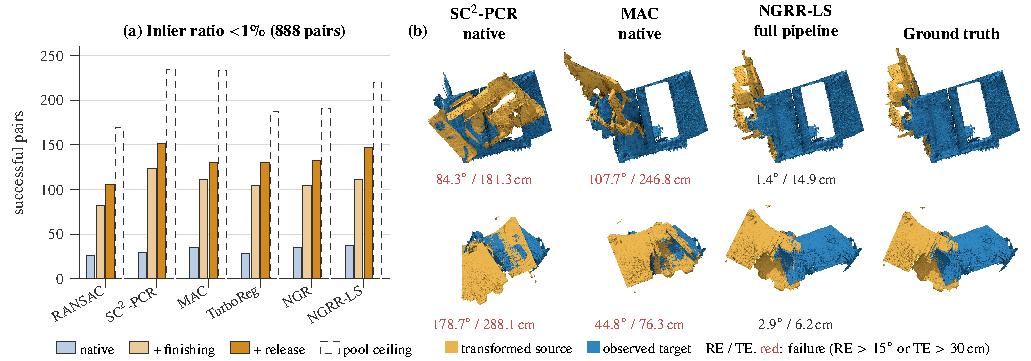
\includegraphics[width=\textwidth]{figures/fig_dilute.pdf}
\caption{(a) All 888 3DLoMatch+FPFH pairs below 1\% inliers: native, finishing, release and refined-pool ceiling. (b) Two recovery cases selected from 97 pairs where the full pipeline succeeds and all four native baselines fail. Panel (a) gives the shared-backend comparison: SC$^2$-PCR registers 152 pairs and NGRR-LS 147.}
\label{fig:dilute}
\end{figure*}



{\clubpenalty=10000\widowpenalty=10000
\Cref{fig:dilute} examines 888 3DLoMatch+FPFH pairs with fewer than 1\% inliers. Native outputs register 26 to 37 pairs, finishing registers 82 to 124, and release registers 106 to 152. NGRR-LS increases from 37 to 147. Among the 381 pairs with 11 to 25 true inliers, it registers 51, the highest count among the six frontends with the common backend. With at most ten inliers, all methods register 3 to 4 of 250 pairs.\par}


In the time--accuracy plane of \cref{fig:pareto}, NGRR-LS with the backend has higher recall and a lower median time than the other original baseline frontends in \cref{tab:main}, with or without the backend.

\begin{figure}[t]
\centering
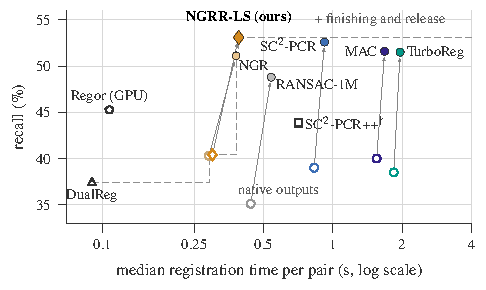
\includegraphics[width=\columnwidth]{figures/fig_pareto.pdf}
\caption{Recall on all 1781 3DLoMatch+FPFH pairs against the median registration-stage time on the 100-pair timing subset (16 CPU threads, MAC 12; \cref{tab:main}). Hollow: native output. Filled: the same frontend with the common finishing and release. Square, triangle, pentagon: native SC$^2$-PCR++, DualReg, Regor (GPU) on the same inputs. $^\dagger$: GPU recall with separate CPU timing. Dashed: CPU Pareto front, excluding $^\dagger$ and Regor. NGRR-LS with the backend has the highest recall; every faster baseline reaches at most 45.3\%.}
\label{fig:pareto}
\end{figure}
